\section{Cubic Subspace Instance Construction}
\frame{\tableofcontents[currentsection]}


\begin{frame}
    \frametitle{Plane and Point Generation}
    \begin{figure}[ht]
        \begin{minipage}{0.5\textwidth}
            \textbf{Plane Generation:}
            \begin{itemize}
                \onslide<1->{
                \item generate 3 planes\\
                as distinct normal vectors $\vec{n}_1, \vec{n}_2, \vec{n}_3$ (normalized)
                }
                \onslide<2->{
                \item compute a $\vec{r}_{i,1}$ (normalized) orthogonal to $\vec{n}_i$
                ($i \in \{1,2,3\}$)
                }
                \onslide<3->{
                \item compute the $\vec{r}_{i,2}$ (normalized) orthogonal to $\vec{n}_i$ and $\vec{r}_{i,1}$
                }
            \end{itemize}
        \end{minipage}
        \begin{minipage}{0.48\textwidth}
            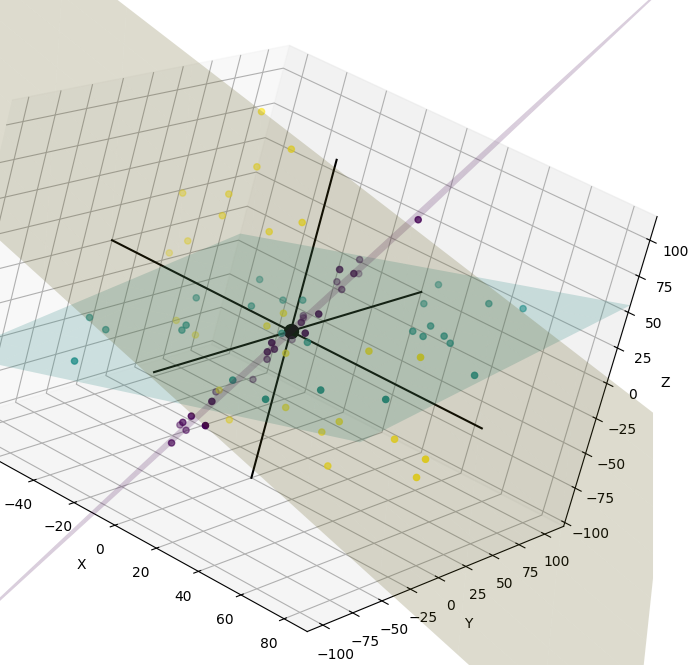
\includegraphics[width=\textwidth]{generated-points.png}
        \end{minipage}
    \end{figure}
    \onslide<4->{
    \textbf{Point Generation} on the plane $(\vec{n},\vec{r}_1,\vec{r}_2)$, parameters $(\maxD,\noise)$:
    \begin{itemize}
        \item random variables $k_1,k_2 \in [-\maxD,\maxD]$ (uniform distribution)
        \item random variable $k_n$ (normal distribution based on $\noise$) 
        \item generate point $p = k_1\vec{r_1} + k_2\vec{r_2} + k_n\vec{n}$ 
    \end{itemize}
    }
\end{frame}


\begin{frame}
    \frametitle{Cost Function (1)}
    % cost function explain what works, wh_at not and why do we need this conditions
    % cost function ~7min with pictures, explain ideas
    % My contribution!!! 
    % Cost function does not depend on the point distribution bounds!!!
    % Steps to assign the cost !!!!!
    % 1. skip triangle where 2 points are close to each other
    % (because may be close to the origin, noise effect, unclear plane spanned by the triangle)
    % 2. skip line like triangles
    % (criteria for almost surely not in the same plane)
    % 3. assign penalty if the noise sum is too large
    \begin{minipage}{0.55\textwidth} 
        \textbf{Triangle} $abc \in \binom{\fSet}{3}$
        \begin{enumerate}
            \onslide<2->{
            \item[(1)] Smallest side $s < \maxD/2$\\
            $\to \cost_{abc} = 0$
            }
            \onslide<3->{
            \item[(2)] Largest angle $\alpha > 150\degree$\\
            $\to \cost_{abc} = 0$
            }
            \onslide<4->{
            \item[(3)] $h_a,h_b,h_c$: distances\\
            to the best fitted plane\\
            containing the origin;\\
            $h_a + h_b + h_c > 3\noise + \tol$\\
            \vspace{5px}
            $\to \cost_{abc} = \frac{(h_a + h_b + h_c) - (3\noise + \tol)}{3\maxD}$
            \vspace{5px}
            }
            \onslide<5->{
            \item[(4)] $h_o$: distance from the origin\\
            to the triangle plane;\\
            $h_o > \frac{10}{\#points}\noise + \tol$\\
            \vspace{5px}
            $\to \cost_{abc} = 0$
            }
        \end{enumerate}
    \end{minipage}
    \begin{minipage}{0.43\textwidth}
        \onslide<2->{
            \begin{tikzpicture}[node distance=30px]
                % nodes
                \node[state, draw=red] (a) {a};
                \node[state, draw=blue] (b) [above right of=a] {b};
                \node[state, draw=blue] (c) [below right of=b] {c};
                \node[state] (o) [above left of=b] {o};
                % edges
                \path[-, ] (a) edge node {} (b);
                \path[-] (b) edge node {} (c);
                \path[-] (c) edge node {} (a);
                \path[-, dashed] (o) edge[red] node {} (a);
                \path[-, dashed] (o) edge[blue] node {} (b);
                
            \end{tikzpicture}
            \hspace{10px}
            \begin{tikzpicture}[node distance=30px]
                % nodes
                \node[state, draw=blue] (a) {a};
                \node[state, draw=blue] (b) [above right of=a, right=10px] {b};
                \node[state, draw=blue] (c) [above right of=a] {c};
                % edges
                \path[-, ] (a) edge node {} (b);
                \path[-] (b) edge node[above] {\small$\noise$} (c);
                \path[-] (c) edge node {} (a);
            \end{tikzpicture}
        }

        \vspace{10px}
        \onslide<3->{
            \begin{tikzpicture}[node distance=30px]
                % nodes
                \node[state, draw=red] (a) {a};
                \node[state, draw=blue] (b) [right of=a, above=7px, right=10px] {b};
                \node[state, draw=blue] (c) [right of=a, right=60px] {c};
                % edges
                \path[-, ] (a) edge node {} (b);
                \path[-] (b) edge node {} (c);
                \path[-] (c) edge node {} (a);
            \end{tikzpicture}
        }

        \vspace{10px}
        \onslide<4->{
            \begin{tikzpicture}[node distance=30px]
                % nodes
                \node[state] (o) {o};
                \node[state, draw=blue] (a1) [right of=o] {a'};
                \node[state, draw=red] (a) [below of=a1, below=10px] {a};
                \node[state, draw=blue] (b1) [right of=o, right=30px] {b'};
                \node[state, draw=blue] (b) [above of=b1, below=3px] {b};
                \node[state, draw=blue] (c1) [right of=o, right=70px] {c'};
                \node[state, draw=blue] (c) [below of=c1, above=10px] {c};
                % edges
                \path[-, dashed] (o) edge[blue] node {} (a1);
                \path[-, dashed] (a1) edge[blue] node {} (b1);
                \path[-, dashed] (b1) edge[blue] node {} (c1);
                \path[-] (a) edge node {} (b);
                \path[-] (b) edge node {} (c);
                \path[-] (c) edge node {} (a);
                \path[-, dotted] (a) edge node[left] {\small $h_a$} (a1);
                \path[-, dotted] (b) edge node[right=6px, below=-6px] {\small $h_b$} (b1);
                \path[-, dotted] (c) edge node[right] {\small $h_c$} (c1);
            \end{tikzpicture}
        }
        
        \vspace{10px}
        \onslide<5->{
            \begin{tikzpicture}[node distance=30px]
                % nodes
                \node[state] (o) {o};
                \node[state, draw=blue] (o1) [below of=o] {o'};
                \node[state, draw=blue] (a) [right of=o1, right=10px] {a};
                \node[state, draw=blue] (b) [right of=o1, right=30px] {b};
                \node[state, draw=blue] (c) [right of=o1, right=60px] {c};
                
                % edges
                \path[-, dashed] (o1) edge[blue] node {} (a);
                \path[-] (a) edge node {} (b);
                \path[-] (b) edge node {} (c);
                \path[-, dotted] (o) edge node[left] {\small $h_o$} (o1);
            \end{tikzpicture}
        }
    \end{minipage}
\end{frame}
    

\begin{frame}
    \frametitle{Cost Function (2)}
        \begin{minipage}{0.55\textwidth}
            \begin{enumerate}
                \item[(5)] for all points $p$:\\
                $h_p$: distance to the best fitted\\
                plane containing the origin;\\
                \vspace{5px}
                \onslide<2->{
                choose $p$ if\\ $h_p < \noise + \tol \land |\vec{p}| > 0.3\maxD$\\
                }
                \vspace{5px}
                \onslide<3->{
                $h_p'$: distance to the best fitted
                plane to all chosen points $p$\\
                containing the origin;\\ 
                }
                \vspace{10px}
                \onslide<4->{
                $\delta_p := \frac{hp' - (\noise + \tol)}{\maxD}$\\
                \vspace{5px}
                $M := \{p \mid p \text{ chosen } \land \delta_p < 0\}$    
                }
                \vspace{10px}
                \onslide<5->{
                $|M| \leq 3 \to \cost_{abc} = 0$\\
                }
                \vspace{10px}
                \onslide<6->{
                $\to \cost_{abc} = 2^{|M|-4} \cdot \sum\limits_{p \in M} \delta_p$    
                }
            \end{enumerate}
        \end{minipage}
        \begin{minipage}{0.43\textwidth}
            \centering
            \begin{tikzpicture}[node distance=30px]
                % nodes
                \node[state] (o) {o};
                \node[state, draw=blue] (a1) [right of=o, right=10px] {a'};
                \node[state, draw=blue] (a) [below of=a1, above=10px] {a};
                \node[state, draw=blue] (b1) [right of=o, right=50px] {b'};
                \node[state, draw=blue] (b) [above of=b1, below=3px] {b};
                \node[state, draw=blue] (c1) [right of=o, right=80px] {c'};
                \node[state, draw=blue] (c) [below of=c1, above=10px] {c};
                \node[state, draw=blue] (p1) [right of=o,left=5px] {p'};
                \node[state] (p) [above of=p1] {p};
                % edges
                \path[-, dashed] (o) edge[blue] node {} (p1);
                \path[-, dashed] (p1) edge[blue] node {} (a1);
                \path[-, dashed] (a1) edge[blue] node {} (b1);
                \path[-, dashed] (b1) edge[blue] node {} (c1);
                \path[-] (a) edge node {} (b);
                \path[-] (b) edge node {} (c);
                \path[-] (c) edge node {} (a);
                \path[-, dotted] (a) edge node {} (a1);
                \path[-, dotted] (b) edge node {} (b1);
                \path[-, dotted] (c) edge node {} (c1);
                \path[-, dotted] (p) edge node[left] {\small $h_p$} (p1);
            \end{tikzpicture}
            \vspace{20px}
            \onslide<3->{
            \begin{tikzpicture}[node distance=30px]
                % nodes
                \node[state] (o) {o};
                \node[state, draw=blue] (p1x) [right of=o,left=5px] {$p_1'$};
                \node[state, draw=blue] (p1) [above of=p1x] {$p_1$};
                \node[state, draw=blue] (p2x) [right of=o, right=10px] {$p_2'$};
                \node[state] (p2) [above of=p2x, above=5px] {$p_2$};
                \node[state, draw=blue] (p3x) [right of=o, right=30px] {$p_3'$};
                \node[state, draw=blue] (p3) [below of=p3x, above=10px] {$p_3$};
                \node[state, draw=blue] (p4x) [right of=o, right=60px] {$p_4'$};
                \node[state, draw=blue] (p4) [above of=p4x, below=5px] {$p_4$};
                \node[state, draw=blue] (p5x) [right of=o, right=80px] {$p_5'$};
                \node[state, draw=blue] (p5) [below of=p5x] {$p_5$};
                % edges
                \path[-, dashed] (o) edge[blue] node {} (p1x);
                \path[-, dotted] (p1) edge node[left] {\small $h_{p_1}'$} (p1x);
                \path[-, dashed] (p1x) edge[blue] node {} (p2x);
                \path[-, dotted] (p2) edge node[left] {\small $h_{p_2}'$} (p2x);
                \path[-, dashed] (p2x) edge[blue] node {} (p3x);
                \path[-, dotted] (p3) edge node[right=1px] {\small $h_{p_3}'$} (p3x);
                \path[-, dashed] (p3x) edge[blue] node {} (p4x);
                \path[-, dotted] (p4) edge node[left] {\small $h_{p_4}'$} (p4x);
                \path[-, dashed] (p4x) edge[blue] node {} (p5x);
                \path[-, dotted] (p5) edge node[left] {\small $h_{p_5}'$} (p5x);
            \end{tikzpicture}
            }
        \end{minipage}
\end{frame}